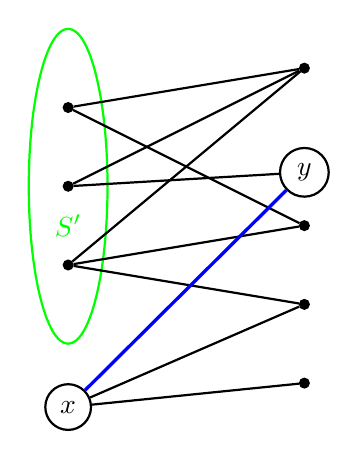
\begin{tikzpicture}[
  dot/.style = {
    shape = circle,
    fill = black,
    minimum size = 4pt,
    inner sep = 0pt,
    outer sep = 0pt,
  },
  every path/.style = {
    thick
  }
]
  \draw[color = green] (0, 2) ellipse (0.5cm and 2cm);
  \draw[color = green] node at (0, 1.5) {\(S'\)};

  \draw node[dot] (L1) at (0, 3) {};
  \draw node[dot] (L2) at (0, 2) {};
  \draw node[dot] (L3) at (0, 1) {};
  \draw node[below, circle, draw = black] (L4) at (0, -0.5) {\(x\)};

  \draw node[dot] (R1) at (3, 3.5) {};
  \draw node[below, circle, draw = black] (R2) at (3, 2.5) {\(y\)};
  \draw node[dot] (R3) at (3, 1.5) {};
  \draw node[dot] (R4) at (3, 0.5) {};
  \draw node[dot] (R5) at (3, -0.5) {};

  \draw (L1) edge (R1) edge (R3);
  \draw (L2) edge (R1) edge (R2);
  \draw (L3) edge (R1) edge (R3) edge (R4);
  \draw (L4) edge (R4) edge (R5);
  \draw[very thick, color = blue] (L4) -- (R2);
\end{tikzpicture}
